\documentclass[10pt,a4paper]{article}

\usepackage[table]{xcolor}
\usepackage[top=20mm, bottom=30mm, left=18mm, right=18mm]{geometry}
\usepackage{multirow}
\usepackage{amsmath}
\usepackage{hyperref}  % Enables hyperlinks

% Encoding
%--------------------------------------
\usepackage[utf8]{inputenc}
\usepackage[T1]{fontenc}
%--------------------------------------
%Portuguese-specific commands
%--------------------------------------
\usepackage[portuguese]{babel}
%--------------------------------------

\definecolor{light_gray}{RGB}{235, 235, 235}

\usepackage{graphicx}
\graphicspath{{./img/}}

\newcommand{\horrule}[1]{\rule{\linewidth}{#1}}

%----------------------------------------------------------------------------------------
%	TITLE SECTION
%----------------------------------------------------------------------------------------

\title{
	\usefont{OT1}{bch}{b}{n}
	\normalfont \Large \textsc{Universidade Federal de Santa Catarina\\
		Departamento de Informática e Estatística\\
		Inteligência Artificial
	} \\ [25pt]
	\horrule{0.5pt} \\[0.4cm]
	\huge Trabalho sobre Métodos de busca \\
	\horrule{2pt} \\[0.5cm]
}

\author{Leonardo V. Eichstaedt\\
        \and
        Makhles Reuter Lange
}
\date{\today}

\begin{document}
\maketitle

%----------------------------------------------------------------------------------------
%	ESTRUTURAS DE DADOS
%----------------------------------------------------------------------------------------

\section{Estruturas de dados escolhidas}

Escolheu-se representar o tabuleiro como uma matrix quadrada de tamanho 15. Sabe-se que no início do jogo e em boa parte deste, a maior parte das casas em que se pode jogar estará vazia e, se nenhum outro tipo de estrutura que determine quais casas devem ser verificadas no cálculo da heurística, há um disperdício de processamento, porém nesta primeira implementação ainda não se está considerando a otimização das computações, pois a heurística ainda está sendo formulada e não há uma implementação efetiva desta. A matriz pode ser vista no construtor da classe \texttt{Board}:
%
\begin{verbatim}
class Board():
    BoardWidth = 15
    BoardHeight = 15

    def __init__(self):
        self.board = [[0 for i in range(self.BoardWidth)] for ii in range(self.BoardHeight)]
        self.pieces = 0

    ...
\end{verbatim}

Uma estrutura a ser considerada é a utilização de um \emph{hash map} que mapeie posições ocupadas às pedras que as ocupam. Nesse caso, tem-se um ganho no consumo de memória utilizada, pois apenas as posições efetivamente ocupadas por pedras brancas ou pretas fazem parte do mapeamento, porém não há nenhum ganho em processamento, visto que uma matriz quadrada de tamanho 15 pode ser armazenada tranquilamente em uma memória cache.

Pensa-se ainda em criar quatro listas referentes às direções de percorrimento do tabuleiro a partir de qualquer pedra: horizontal, vertical e diagonais. Essas listas podem conter as pedras que devem ser percorridas em suas respectivas direções para contabilizar os pontos. Nesse caso, se em uma dada configuração do tabuleiro foi determinado que uma pedra não irá pontuar na direção horizontal (por não haver a possibilidade de se formar uma quíntupla), então essa pedra é removida da lista horizontal. Assim, nas aplicações seguintes da heurística, não há a necessidade de se percorrer horizontalmente a estrutura de dados a partir daquela pedra.



%----------------------------------------------------------------------------------------
%	HEURÍSTICA
%----------------------------------------------------------------------------------------
\newpage
\section{Heurística e utilidade} \label{sec:heuristica}

A função heurística $h(n)$, onde $n$ se refere à configuração do tabuleiro, pode ser composta de diversas outras definições. A principal heurística a ser utilizada nesse trabalho é dada pela Equação~\ref{eqn:heuristic}.

\begin{equation}\label{eqn:heuristic}
h(n) = \sum_{i=1}^{5} 10^{2*i} \times seq_i
\end{equation}
%
onde $seq_i$ representa a quantidade de sequências de $i$ pedras consecutivas ou semi-consecutivas, desde que haja a possibilidade de se alcançar 5 pedras consecutivas. Por exemplo, na configuração $n$ do tabuleiro da Figura~\ref{fig:heuristic}, tem-se:

\begin{equation*}
\begin{split}
h(n) = &10^2 \times (C_{diagonal2} + E_{diagonal1} + F_{vertical} + F_{diagonal2}) + \\
       &10^4 \times (BE_{diagonal2} + DE_{horizontal}) + \\
       &10^6 \times (ABC_{horizontal} + CDF_{diagona1})
\end{split}
\end{equation*}

\begin{equation*}
h(n) =  4 \times 10^2 + 2 \times 10^4 + 2 \times 10^6
\end{equation*}
%
onde \emph{diagonal1} se refere a uma reta de inclinação positiva e \emph{diagonal2} a uma reta de inclinação negativa. 

\begin{figure}[!htbp]
    \centering
        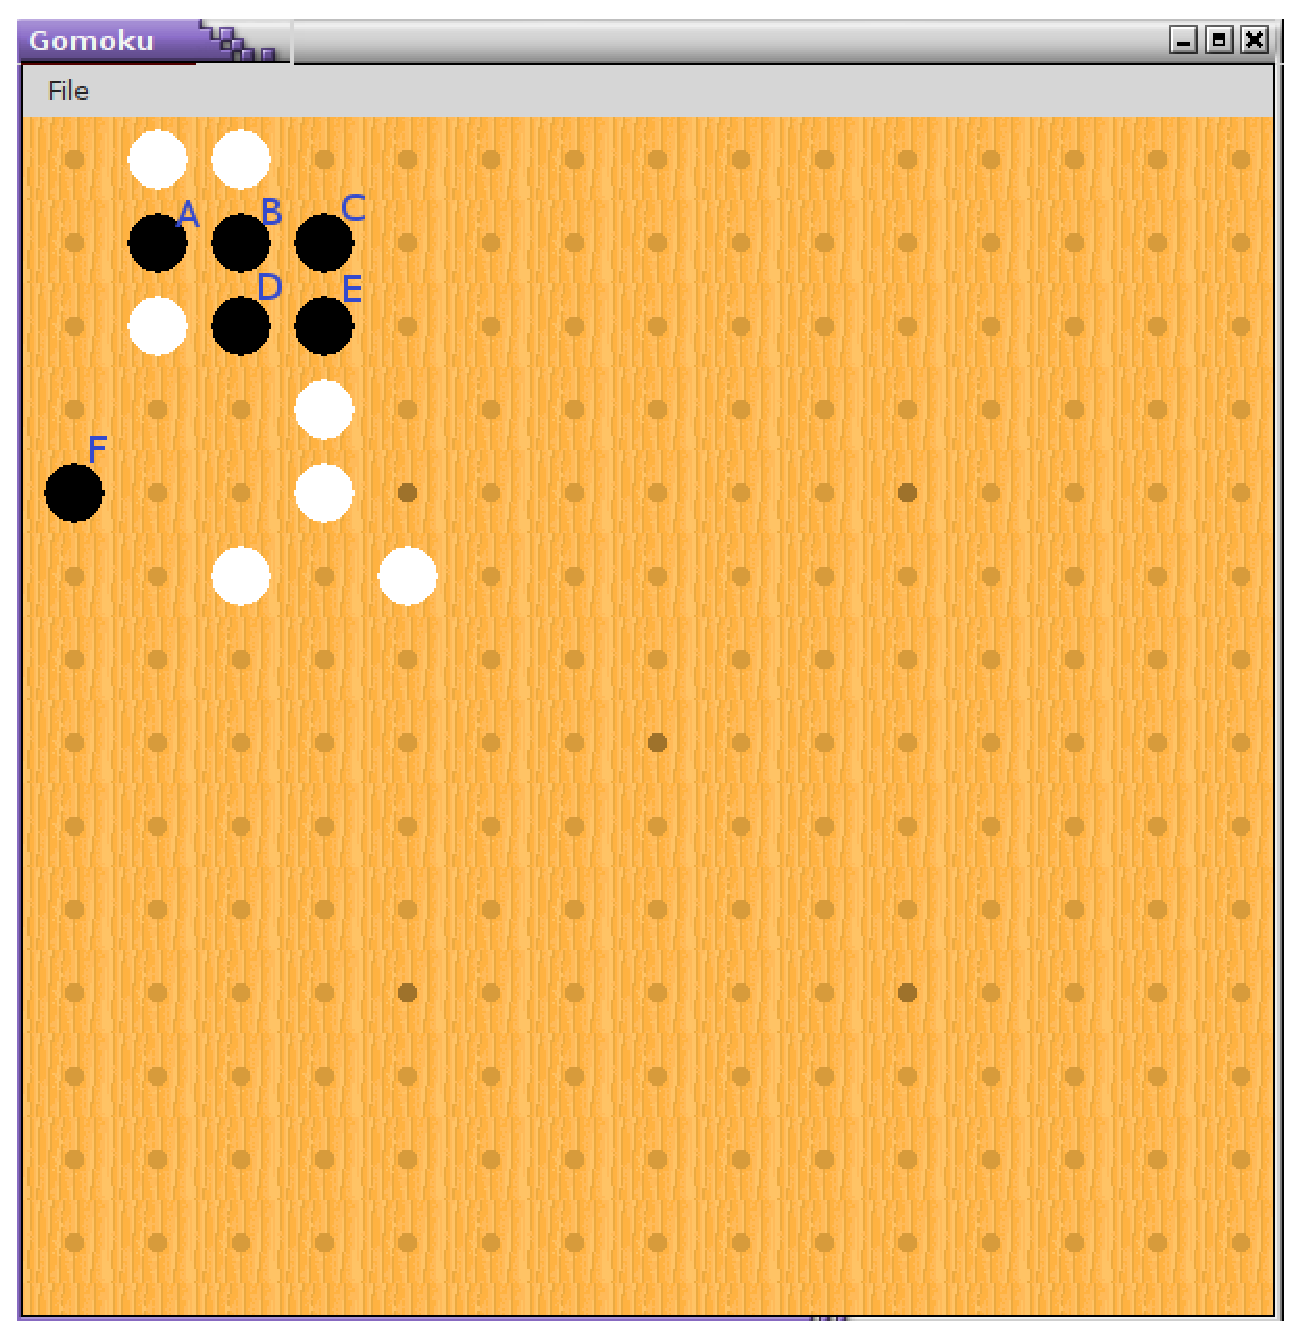
\includegraphics[scale=0.5]{heuristic}
    \caption{Execução do próprio jogo que está sendo desenvolvido.}
    \label{fig:heuristic}
\end{figure}

A implementação da heurística no código ainda está em fase de desenvolvimento. Não se está utilizando os pesos definidos na Equação~\ref{eqn:heuristic} ainda, apenas soma-se um valor de 10 para cada peça em uma sequência, desde que se possa chegar a uma quíntupla.

Futuramente, pensa-se em incluir também alguma maneira de conferir mais pontos às configurações em que se pode preencher 5 pedras com mais de uma forma. Por exemplo, utilizando-se a mesma imagem, a sequência \texttt{ABC} pode gerar as quíntuplas \texttt{xABCx} e \texttt{ABCxx}, o que deve conferir mais pontos que a configuração \texttt{FxDCx}, que é a única forma de se fazer uma quíntupla com as pedras \texttt{C}, \texttt{D} e \texttt{F}.

Tem-se ainda a possibilidade de incluir heurísticas referentes a determinadas configurações de pedras que levarão a uma vitória independentemente da jogada do humano.

Uma outra abordagem a ser considerada é como fazer a pontuação nas situações em que a configuração do tabuleiro está favorável para a AI, porém muito mais favorável para o jogador humano.


%----------------------------------------------------------------------------------------
%	DETECÇÃO DO FIM DE JOGO
%----------------------------------------------------------------------------------------

\section{Detecção do Fim de Jogo} \label{sec:fim_de_jogo}

Nessa implementação parcial do jogo, faz-se a detecção do fim do jogo no método \texttt{checkWin} da classe \texttt{Board}, conforme o trecho de código abaixo apresentado:

\begin{verbatim}
    def checkWin(self, m, n, player):

        count = 1
        self.pieces = self.pieces + 1
        if (self.pieces == 15 * 15):
            return DRAW

        # Vencendo pela diagonal baixo direita
        for i in range(1, 5):
            if (m - i >= 0 and n - i >= 0 and self.board[m - i][n - i] == player):
                count = count + 1
            else:
                break
        if (count == 5):
            return WIN
        else:
            count = 1

        # Vencendo pela diagonal cima direita
        for i in range(1, 5):
            if (m + i <= 14 and n - i >= 0 and self.board[m + i][n - i] == player):
                count = count + 1
            else:
                break
        if (count == 5):
            return WIN
        else:
            count = 1

        # Vencendo pela diagonal baixo esquerda
        for i in range(1, 5):
            if (m - i >= 0 and n + i <= 14 and self.board[m - i][n + i] == player):
                count = count + 1
            else:
                break
        if (count == 5):
            return WIN
        else:
            count = 1

        # Vencendo pela diagonal cima esquerda
        for i in range(1, 5):
            if (m + i <= 14 and n + i <= 14 and self.board[m + i][n + i] == player):
                count = count + 1
            else:
                break
        if (count == 5):
            return WIN
        else:
            count = 1

        # Vencendo pela esquerda
        for i in range(1, 5):
            if (n + i <= 14 and self.board[m][n + i] == player):
                count = count + 1
            else:
                break
        if (count == 5):
            return WIN
        else:
            count = 1

        # Vencendo pela direita
        for i in range(1, 5):
            if (n - i >= 0 and self.board[m][n - i] == player):
                count = count + 1
            else:
                break
        if (count == 5):
            return WIN
        else:
            count = 1

        # Vencendo por Cima
        for i in range(1, 5):
            if (m + i <= 14 and self.board[m + i][n] == player):
                count = count + 1
            else:
                break
        if (count == 5):
            return WIN
        else:
            count = 1

        # Vencendo por Baixo
        for i in range(1, 5):
            if (m - i >= 0 and self.board[m - i][n] == player):
                count = count + 1
            else:
                break
        if (count == 5):
            return WIN
        else:
            count = 1

        return CONTINUE
\end{verbatim}

Conta-se o número de pedras conectadas à pedra recém-jogada e retorna-se um dos seguintes valores:
%
\begin{itemize}
    \item \textbf{CONTINUE} - o jogo está em andamento (retorno padrão);
    \item \textbf{WIN} - o jogo terminou com a vitória de um dos jogadores;
    \item \textbf{DRAW} - o jogo terminou em um empate.
\end{itemize}


%----------------------------------------------------------------------------------------
%	DETECÇÃO DE SEQUÊNCIAS DE 4 PEÇAS
%----------------------------------------------------------------------------------------

%\section{Detecção de Sequências de 4 Peças}




%----------------------------------------------------------------------------------------
%	REFERÊNCIAS BIBLIOGRÁFICAS
%----------------------------------------------------------------------------------------

%\section{Referências Bibliográficas}


\end{document}
